\documentclass[10pt,a4paper]{report}
\usepackage[utf8]{inputenc}
%\usepackage[backend=biber,style=numeric]{biblatex}
\usepackage[backend=biber,style=numeric,sorting=ynt]{biblatex}
\usepackage[english]{babel}
 
\usepackage{graphicx}
\usepackage{multirow}
\usepackage{mathtools}
\usepackage{amsmath}
\usepackage{xcolor}
\usepackage{colortbl}
\usepackage{amsmath,amssymb,amsfonts}
\usepackage{algorithm}
\usepackage{numprint}
\usepackage{listings}
\usepackage{tabu}
\usepackage{enumitem}

\addbibresource{main.bib}

\title{\centering \textbf{Second Year Review\thanks{Progress report and thesis vision}}\\Towards Alleviating The Task of Software Parallelization}
\author{Aleksandr Maramzin\\s1736883}
\date{June 2020}

\lstdefinestyle{mystyle}{
  backgroundcolor=\color{white},   % choose the background color; you must add \usepackage{color} or \usepackage{xcolor}; should come as last argument
  basicstyle=\ttfamily\footnotesize,        % the size of the fonts that are used for the code
  breakatwhitespace=false,         % sets if automatic breaks should only happen at whitespace
  breaklines=true,                 % sets automatic line breaking
  captionpos=b,                    % sets the caption-position to bottom
  commentstyle=\itshape\color{green},    % comment style
  deletekeywords={...},            % if you want to delete keywords from the given language
  escapeinside={\%*}{*)},          % if you want to add LaTeX within your code
  extendedchars=true,              % lets you use non-ASCII characters; for 8-bits encodings only, does not work with UTF-8
  firstnumber=1000,                % start line enumeration with line 1000
  % frame=single,	                   % adds a frame around the code
  keepspaces=true,                 % keeps spaces in text, useful for keeping indentation of code (possibly needs columns=flexible)
  keywordstyle=\color{blue},       % keyword style
  language=C,                 % the language of the code
  morekeywords={*,...},            % if you want to add more keywords to the set
  numbers=none,                    % where to put the line-numbers; possible values are (none, left, right)
  numbersep=5pt,                   % how far the line-numbers are from the code
  numberstyle=\tiny\color{grey}, % the style that is used for the line-numbers
  rulecolor=\color{black},         % if not set, the frame-color may be changed on line-breaks within not-black text (e.g. comments (green here))
  showspaces=false,                % show spaces everywhere adding particular underscores; it overrides 'showstringspaces'
  showstringspaces=false,          % underline spaces within strings only
  showtabs=false,                  % show tabs within strings adding particular underscores
  stepnumber=2,                    % the step between two line-numbers. If it's 1, each line will be numbered
  stringstyle=\color{purple},      % string literal style
  tabsize=2,	                   % sets default tabsize to 2 spaces
  title=\lstname                   % show the filename of files included with \lstinputlisting; also try caption instead of title
}

\lstset{style=mystyle}

\begin{document}

\maketitle

\begin{abstract}

% Problem: the need for manual parallelization has not yet gone away, despite decades of work automatic parallelization tools do not deliver desired performance improvements

\quad Parallel hardware has become ubiquitous through the entire spectrum of computing systems, from low-end embedded devices to high-end supercomputers. Yet, most of the existing software is written in a sequential fashion: be it an old legacy software initially designed to run on the available at that time serial hardware or modern applications being developed by application domain experts rather than performance engineers. In order to exploit all available hardware facilities software has to be parallelized.\newline\null
\quad The problem of software parallelization is extremely complex and multifaceted and requires of programmers to possess an additional (apart from their application domain expertise) knowledge in various domains of parallel programming (from cache coherence protocols to high level algorithmic skeletons). For decades researches and engineers have been working on automatic parallelization techniques, which are supposed to ultimately liberate programmers from the challenging task of manual parallelisation. But, despite the massive body of work on the subject, automatic techniques still cannot deliver performance levels expert programmers reach and are limited to narrow domains of scientific Fortran codes and relatively simple computational idioms.\newline\null
\quad Given the difficulty of the obstacles faced by automatic parallelisation today, we do not expect a breakthrough in the area or a "silver bullet" solving the problem in the near future. We acknowledge the role of a human expert, but at the same time we propose an assistant solution, which can be used to guide programmer's efforts and alleviate the manual parallelisation task.\newline\null
\quad The assistant solution we propose is as multifaceted as the problem itself and consists of several components aimed to tackle different aspects of software parallelisability. It is a toolkit rather than a single tool. The first tool in the toolkit has been designed, developed and assessed during the first year of my PhD. Complementary tools are supposed to be developed over the course of remaining time.\newline\null
\quad The designed tool is basically a machine learning (ML) based model of loop parallelisability integrated and utilised into an assistant scheme. Assistant takes an application to be parallelised along with its profile as an input and presents a programmer with a ranking of application loops. In contrast to a profile guided approach, assistant's ranking highlights application loops, which are not only long-running (and thus potentially profitable), but crucially parallelisable. This way a programmer concentrates his efforts on promising application loops and converges to the best achievable performance faster. We have deployed our assistant on SNU NAS Parallel Benchmarks \cite{snu-npb-benchmarks} \cite{nasa-parallel-benchmarks} and demonstrated a potential of our idea \cite{aiseps}.\newline\null
\quad The second tool we want to add to our software parallelisation toolkit solution is aimed at addressing the problem of unsuccessful data structure choice, which might turn a perfectly parallelisable at a higher level computation into a non-parallelisable lower level implementation. The tool is at the literature review and feasibility study stage.
\end{abstract}

\chapter{Thesis Vision\\{\Large Research Path}}
\quad In our work we address the topic of \textbf{software parallelization}. Software parallelization is a multifaceted and complex task. A perfectly decomposable and parallelizable problem might end up being implemented with an unsuccessfully chosen non-parallelizable algorithm. And the algorithm in its turn might end up being implemented with an unsuccessfully chosen lower level constructions such as pointers, heap-allocated and pointer-linked data structures, indirect array referencing, etc. Legacy source code bases have been designed primarily for serial machines and are rich with all these sub-optimal from the angle of software parallelization programming decisions.\newline\null
\quad Despite decades of research into parallelizing compiler technology, the latter still fails to tackle real world legacy code challenges and software parallelization remains a largely manual task where the key resource is expert time. We do not strive to find a "silver bullet", instead we acknowledge the role of a programmer in the software parallelization process and aim at alleviating the task.\newline\null
\quad The work started during my MSc by Research year with an idea of "Software Metrics for Parallelism". The idea was based on the similar work in the field of software quality metrics. Cyclomatic complexity (CC) software metric might be taken as an illustrative example, which quantitatively characterizes the difficulty of program comprehension. The idea of "Software Metrics for Parallelism" has passed through several stages of lost and revived interest. As we implemented our parallelizability metrics inside the LLVM and finally got to see their behaviour on SNU NPB benchmark suite, we observed the weakness of metrics correlation with software parallelizability property. That was right at the end of my MSc by the Research. Then we decided to use the metrics as machine learning features and created a model of loop parallelizability. The predictive accuracy was initially low causing us to doubt in learnability of that property for the SNU NPB suite. It took us a while before we managed to get an acceptable above 90\% level. At this point we realized that it is not enough to just learn loop parallelizability property. We developed an assistant scheme extending Intel Compiler's parallelism discovery capabilities. But parallelizability does not necessarily materialize into actual performance improvements. We had to create a crafty scheme taking an application profile and using ML model to ultimately point the best loops to concentrate a programmer efforts on. All that resulted into an end-to-end tool assisting a programmer by providing the latter with the best loop ranking to start parallelisation with.\newline\null
\quad But the tool we developed is just a piece in a final solution package we aim to get. The next step would be to tackle the problem of heap allocated pointer linked data structures. At least we would like to develop a tool capable of their recognition (is it a tree or a linked list?, etc). As the literature review section of DCP project and SPEC CPU2006 feasibility studies show, static methods (such as shape analysis o
r Idiom Description Language (IDL) based on a constraint solver) are unlikely to recognize data structures of SPEC CPU complexity level. We need to use dynamic techniques, which would recreate a dynamic model of data structure heap layout. Vast array of recent work in that direction proves that feeling.




Despite decades of research into parallelizing compiler tech-nology, software parallelization remains a largely manualtask where the key resource is expert time. In this paperwe focus on the time-consuming task of identifying thoseloops in a program, which are both worthwhile and feasible to parallelize. We present a methodology and tool whichmake better use of expert time by guiding their effort directlytowards those loops, where the largest performance gainscan be expected while keeping analysis and transformationeffort at a minimum.We have developed a novel parallelization assistant thatprovides programmers with a ranking of all loops in a pro-gram based on their overall merit. For each loop this metriccombines its potential contribution to speedup and an es-timated probability for its successful parallelization. Thisprobability is predicted using a machine learning model,which has been trained, validated, and tested on 1415 la-belled loops, achieving a prediction accuracy greater than90%.We have evaluated our parallelization assistant againstsequential C applications from the SNU NAS benchmarksuite. We show that our novel methodology achieves par-allel performance levels comparable to those from expertprogrammers while requiring less expert time. On average,our assistant reduces the number of lines of code that have to


\quad Efficient software parallelization requires work to be done at several levels of abstraction. A programmer starts at a high algorithmic level and makes decisions on problem decomposition and software architecture.       





\chapter{$2^{nd}$ Year Timeline}
\quad This chapter describes all activities I have been doing during the $2^{nd}$ year of my PhD. Section \ref{active_timeline} maps them onto the year's timeline. Section \ref{active_description} gives detailed descriptions. After passing the first year review I started my second year with the work towards attending AI-SEPS 2019 workshop. After the workshop at the end of October and a meeting with Bjoern I have properly started with the "Data-Centric Parallelisation (DCP)" project. As our SPEC CPU2006 feasibility studies showed it would be extremely difficult to automatically recognise data structures in SPEC CPU2006 benchmarks. Data structures there are entangled with algorithms and spread across the whole source code base.          


I started the second year of my PhD with passing the first year review and starting to work towards presenting my work on "Machine Learning Based Software Parallelisation Assistant (ML assistant)" at AI-SEPS2019 workshop. After the attendance of the workshop at the end of October I have completely switched onto the "Data-Centric Parallelisation (DCP)" project I started to work on during the previous year. Having finished the literature review for the DCP project and having looked at the SPEC CPU2006 benchmark it has been concluded, that we need a simpler set of benchmarks for the work to be feasible. I spent the whole November and December studying several of Olden benchmarks and writing reports on them from the point of data structure recognition and abstraction level lifting. At around Christmas the notion of the Fractal has been coined inspired by the computations and data structures present at several Olden benchmarks. And since that time I started to work  


In January I have rewritten the health benchmark with the first            


   
\section{The Timeline of My Second Year Activities}
\label{active_timeline}
\begin{description}[style=nextline]
\item [Sep (Annual Review and AI-SEPS 2019 presentations)]\hfill
\begin{itemize}
%\renewcommand\labelitemi{$\vartriangleright$}
\renewcommand\labelitemi{$\bullet$}
\item $1^{st}$ Year Review Presentation and Meeting 
\item AI-SEPS 2019 visa paperwork
\item Work on AI-SEPS 2019 presentation
\end{itemize}
\item [Oct (AI-SEPS 2019 workshop)]\hfill
\begin{itemize}
%\renewcommand\labelitemi{$\vartriangleright$}
\renewcommand\labelitemi{$\bullet$}
\item Work on AI-SEPS 2019 presentation
\item Travel planning and paperwork 
\item Attending AI-SEPS 2019 workshop
\end{itemize}
\item [Nov (Olden benchmarks study)]\hfill
\begin{itemize}
%\renewcommand\labelitemi{$\vartriangleright$}
\renewcommand\labelitemi{$\bullet$}
\item Writing documents on Olden benchmarks 
\item Studying the source code of Olden benchmarks (mst, tsp, perimeter, health, power, treeadd)
\end{itemize}
\item [Dec (LibTooling reading and writing toy examples)]\hfill
\begin{itemize}
\renewcommand\labelitemi{$\bullet$}
\item Reading on Clang LLVM and LibTooling
\item Writing and compiling toy examples with arrays and linked-lists
\item Studying the source code of Olden benchmarks (mst, tsp, perimeter, health, power, treeadd)
\item Christmas break
\end{itemize}
\item [Jan (The idea of the Fractal)]\hfill
\begin{itemize}
\renewcommand\labelitemi{$\bullet$}
\item Developed and designed a Fractal class template
\item Rewrote health benchmark with the Fractal template and got 20\% performance improvement
\item Paper on Tree Accumulations as the theoretical foundation for Fractal
\end{itemize}
\item [Feb (Fractal redesign)]\hfill
\begin{itemize}
\renewcommand\labelitemi{$\bullet$}
\item Rewrote Fractal class template 
\item Rewrote perimeter and treeadd Olden benchmarks to use the new Fractal class
\end{itemize}
\item [Mar (Fold and Reduce computational frameworks)]\hfill
\begin{itemize}
\renewcommand\labelitemi{$\bullet$}
\item ResearchFish report writing
\item Work on the power Olden benchmark
\item Work on Fold and Reduce frameworks 
\end{itemize}
\item [Apr (Fold and Reduce computational frameworks)]\hfill
\begin{itemize}
\renewcommand\labelitemi{$\bullet$}
\item Work on Fold and Reduce frameworks
\item Redesign of Fractal framework for coherence with Fold and Reduce
\item Work on the power benchmark
\end{itemize}
\item [May]\hfill
\begin{itemize}
\renewcommand\labelitemi{$\bullet$}
\item Thesis writing
\item [Reading] Software architecture design patterns
\item Work on the library as the whole
\end{itemize}
\item [Jun (Second Year Report Writing)]\hfill
\begin{itemize}
\renewcommand\labelitemi{$\bullet$}
\item Thesis writing
\item Second Year Report writing
\item Work on the library as the whole
\end{itemize}
\end{description}

\section{Description of Activities}
\label{active_description}
\quad During the $2^{nd}$ year of my PhD I continued to work towards the "Data-Centric Parallelization (DCP)" project. In the previous year we conducted a feasibility study on SPEC CPU2006 benchmarks as an initial step towards the automatic data structure recognition and source code rejuvenation. That created the ground for this year's work. Looking at the real world code of SPEC CPU2006 benchmarks we have learnt some things regarding the problem we are tackling. A more detailed report can be found in section \ref{spec_cpu2006_feasibility}.
\begin{description}[style=nextline]
\item [Research interest] Some of the SPEC CPU2006 benchmarks present an interest from the angle of data structures and algorithmic skeletons recognition.\hfill
\item [Real world legacy code complexity] SPEC CPU2006 benchmarks are extremely complex. It requires a serious effort to comprehend and manually rewrite them with an alternative implementation. Automatic static techniques seem infeasible, while dynamic techniques seem to be a grand challenge.\hfill
\item [Close relationship between algorithms and data structures] Unfortunately, it is quite common in the real world legacy code to see data structures, their update and manipulation operations and the main application algorithms to be entangled together in a same chunk of code. Moreover, functionality pieces are often spread all around the code base. Sometimes, algorithms and data structures are logically inseparable. That makes the motivating case for the creation of computational frameworks as the notion unifying data structures and algorithms together.\hfill
\end{description}
\quad Following the SPEC CPU2006 feasibility study we moved onto another suite of benchmarks. Olden benchmarks are smaller and simpler, but at the same time represent the real world legacy code with all its problems. Throughout the year I have been working the the suite doing the following: 
\begin{itemize}
\renewcommand\labelitemi{$\bullet$}
\item Olden benchmarks study
\item Computational frameworks library design
\item Olden benchmarks rewriting
\item Thesis writing
\end{itemize}
\quad All the above tasks are interdependent and happened iteratively and in close cooperation with one another.
\subsection{Olden benchmarks study}
\label{olden_benchmarks_study}
\quad Olden benchmark suite consists of 10 benchmarks. I have looked at 6 of those (bisort, health, perimeter, treeadd, mst and tsp benchmarks). 


The nature of different Olden benchmarks varies. Benchmarks health, treeadd and perimeter perform basically the same computation. Benchmarks tsp and mst solve 2 well-known graph problems.  

Loops withing these benchmarks work on multidimensional arrays, are highly parallelisable (some need function inlining to be done upfront) and resemble each other. 

Parallelisability?

\paragraph{bisort}
\textit{\textbf{Definition} A sorted sequence is a monotonically non-decreasing (or non-increasing) sequence. A bitonic sequence is a sequence with $x_{0} \leq ... \leq x_{k} \geq ... \geq x_{n}−1$ for some k, or a circular shift of such a sequence.}\newline\null
\quad The sequence is based on a binary tree implementation (recursive calls to left and right subtrees). The algorithm is based on a sorting comparator network consisting of several layers. The network can be and is implemented in a divide and conquer way similar to that of a well-known merge sort. Sort() function is called on the left and right array halves recursively. The merging step of the merge sort algorithm is substituted with compare-and-swap step. The latter is possible due to input sequences required to be bitonic.
\quad\textbf{The benchmark is heavily based on pointers, tree swaps and rotations. It presents an interest from the point of divide and conquer algorithm recognition. Static techniques are unlikely to handle the legacy source code of that complexity and style. Dynamic techniques sould be able to see the binary tree.}      

\paragraph{health} The most promising of all Olden benchmarks. Columbian health care system simulation is based on a complete 4-ary tree of $4^{max_level}$ adjacent villages. Each village has its own hospital and is connected to 4 adjacent child villages. Simulation starts from the top (tree root village and goes down all the tree branches recursively right to left.
Every simulation step consists of several events:
1) Accept all patients from adjacent villages and put them in the local hospital for an initial assessment and possibly for further hospitalization inside the local hospital. 
2) Check patients who are inside the local hospital: once inside patients spend time to recover and occupy 1 member of the staff throughout all time. If time have passed then the patient is checked out and releases 1 personnel member.
3) Check patients on the assessment list. Patients require some time to be diagnosed. Each patient occupies 1 member of the staff throughout the whole assessment process. If patient is ill then he continues to occupy the same personnel member and goes inside the hospital. If patient is healthy the the patient is checked out and releases 1 staff member.
4) Check patients on the waiting list. Once a patient gets into the hospital he/she takes on 1 member of the staff if the personnel is
available. If not, then the patient goes onto the waiting list. Patient passes through 2 phases: assessment and hospitalisation. Each patient is being supervised by 1 member of the personnel starting from assessment and up until checking out of the hospital. If after assessment a patient turns out to be healthy then the patient is checked out and a personnel member is returned back to available pool. If patient is confirmed ill, then the former is put inside the hospital and spends time there. Patients fall ill at the will of a random number generator. 
\quad The benchmark operates with quad tree structures and does it in a highly parallel fashion. In our work we call that pattern a fractal. The latter is a computational framework, i.e. the blend of an algorithm and a data structure. The whole structure can be aimed at for an automatic recognition (not just a separate tree or an algorithmic skeleton, but both) even with static techniques.

\paragraph{perimeter} The benchmark computes the perimeter of a ring (R=2048, r=1024). The ring is mapped onto a grid of elements by painting all the grid elements inside the ring ($r \lt x*x+y*y \lt R$) as black and all grid elements outside of it as white. Then the grid is being traversed in two different (implementation dependent) ways and detects all flips of color (black to white and vice versa) to sum them up into the final perimeter approximation. The grid is implemented as a quad tree based fractal. The initial square is split into 4 parts (northwest, northeast, southwest, southeast), which in their turn split further on. The process reminds the fractal framework from the health benchmark.  

\paragraph{power} The second by importance is the power pricing computation benchmark. The benchmark is based on a composite structure of C arrays and pointer-based linked lists of various objects such as Root, Laterals, Branches and Leaves. Figure \ref{fig:power_benchmark} illustrates the data structure. The algorithm is basically composed of folds and reductions. C arrays are reduced and linked lists are folded. The algorithm works recursively and starts with the Root::compute() call. The method accumulates power demand
Demand(P,Q) from all lists of Laterals. Accumulation starts with the end of each list. Each lateral accumulates its power demand from all its branches and the latter in turn accumulate power demand from all their leaves. The leaves call
optimize\_node() method, which does a chunk of scientific computations (gradients, vectors, etc.), which compute P and Q. Finally, Root::compute() is called iteratively from a while
loop of power\_pricing\_problem(). Iteration continues up until P and Q error becomes less than the required epsilon. 
\begin{figure}[ht]
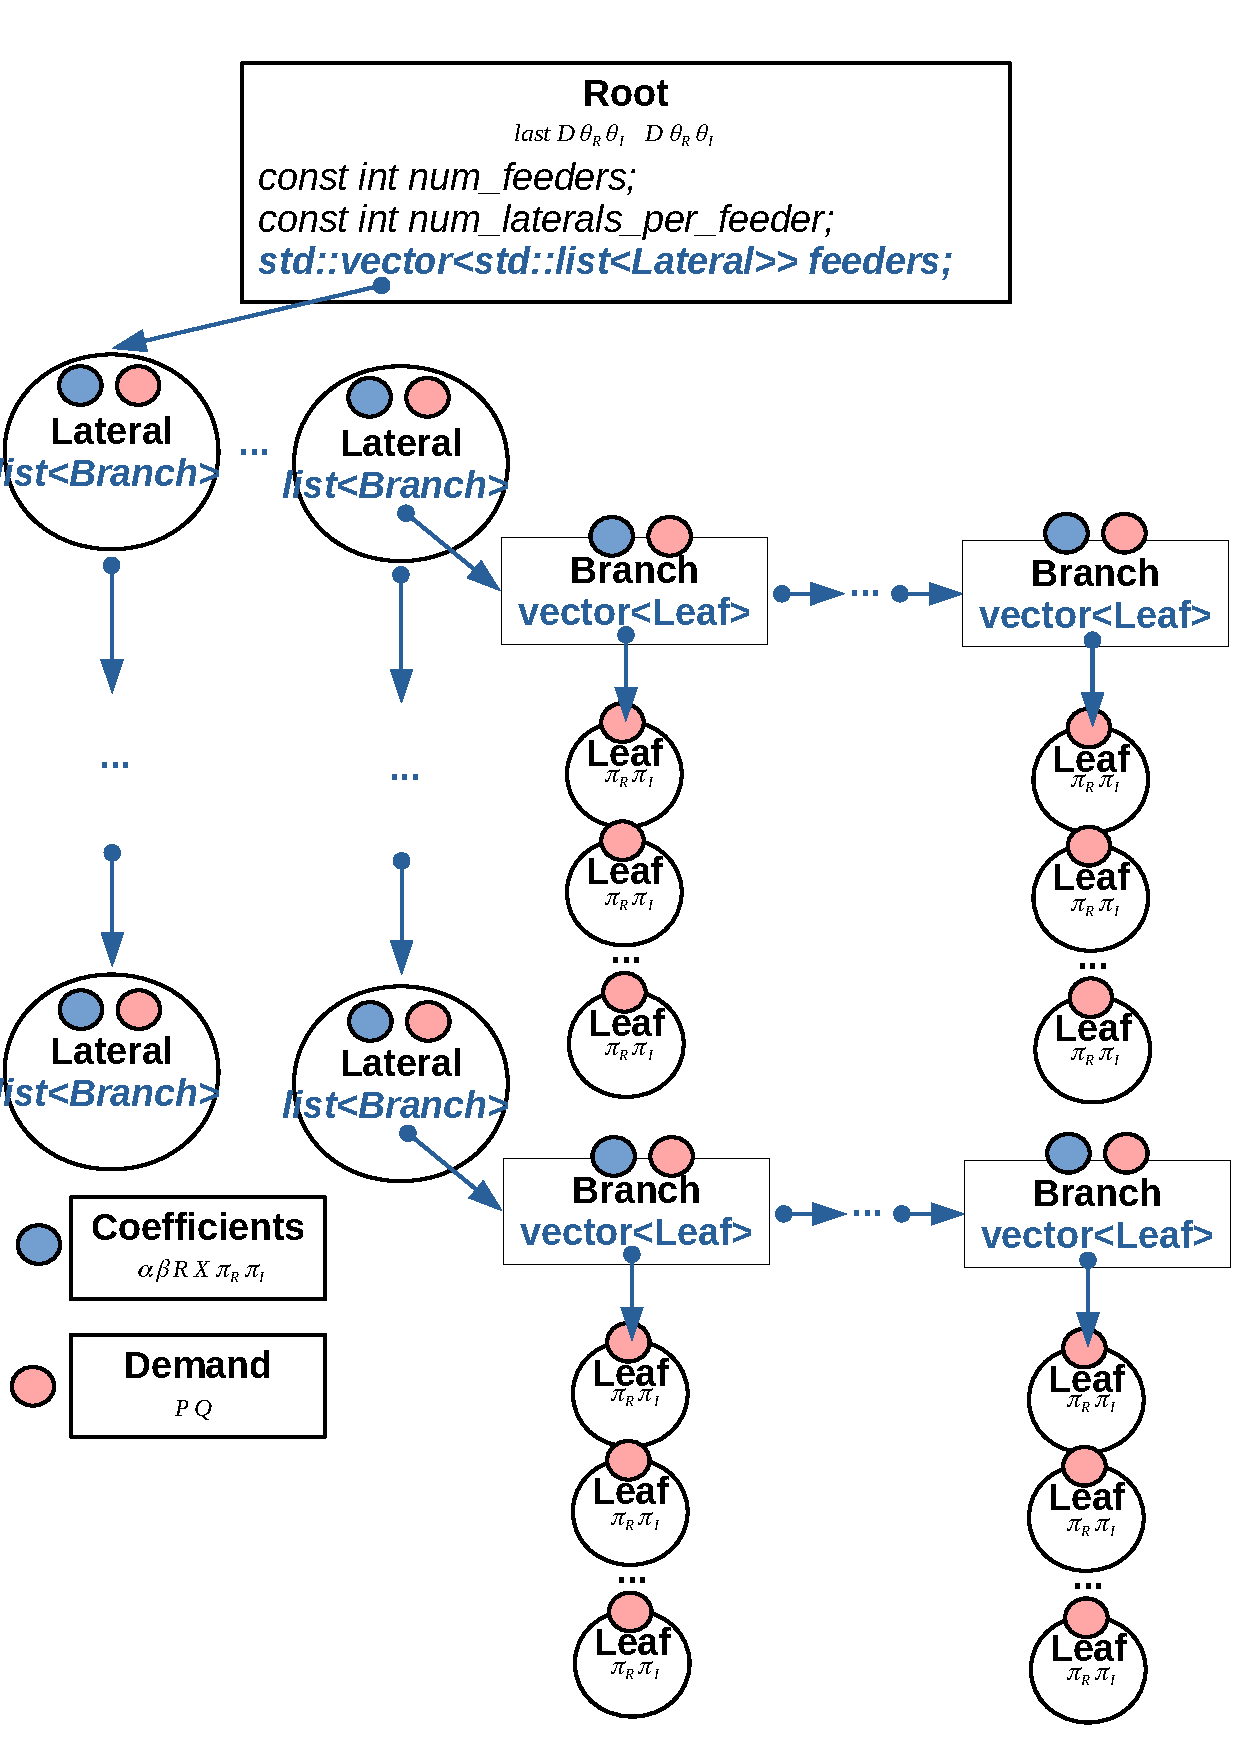
\includegraphics[width=1.0\textwidth]{images/power_scheme.pdf}
\caption{The Power benchmark.}
\label{fig:power_benchmark}
\end{figure}

\paragraph{treeadd}

\paragraph{mst} Minimum Spanning Tree (MST) benchmark does a MST weight computation of a complete graph. Computation is approximate and the algorithm looks like it might finish with incorrect result. Nevertheless, the benchmark can be used for the purpose of computational workload. Graph is represented as a linked list of vertices. Every node in the list has a hash table of incident edges. Graph is complete: each vertex is connected to all other vertices in the graph (except itself). Algorithm repeatedly traverses the list of vertices and gradually accumulates the MST weight. On every traversal algorithm picks the node in the list to use as an input for the next traversal. In that sense, there is a cross iteration/traversal dependency. The code below summarises the benchmark.\newline\null
\begin{minipage}[t]{\linewidth}
\begin{lstlisting}[caption={The main algorithm of mst benchmark.},label={lst:mst_code},language=C]
vertex = list;
list = list->next;
while (num_vertices) {
    ret = traverse_vertex_list(vertex, list);
    mst_weight += ret.distance; // accumulate the final result
    vertex = ret.vertex; // next vertex to measure the distance against
    num_vertices--;
}
return mst_weight;
\end{lstlisting}
\end{minipage}


\paragraph{tsp} Travelling Salesman Problem (TSP). The benchmark generates a set of dots scattered on a 2D plane. Dots represent cities and are specified by their (x,y) coordinates. The TSP problem is to visit all the cities and return to the city of origin having passed the minimal distance. In other words, the algorithm returns a cycled sequence of cities, where proximity of elements in the sequence in terms of order means their spatial proximity on the 2D plane.\newline\null
\quad The algorithm’s work resembles that of an insertion sort. The sequence is divided into 2 parts. Ordered part and unordered part. At first, ordered part consists of just 1 element. On every iteration the algorithm takes the next element out of unordered part, finds it a pairing element inside the ordered part (with the minimal distance between them) and inserts the element into the ordered subsequence next to its pair. At the end we get the sequence with the property that closest dots stand the closest in the sequence.\newline\null
\quad The benchmark is based on a binary tree being transformed into doubly linked list. 

Computational method

1) A binary tree is built. Every node of the tree represents a city located on 2D plane with randomly generated (x,y) coordinates. The build\_tree() method is written in a way to generate a uniform distribution of dots on the plane.


\paragraph{Computational Frameworks library development}
\quad As any software development process, the development of the library happened iteratively and non-linearly. The development started with the concept of \textbf{fractal} gleaned out of the algorithm and data structure commonalities among health, perimeter and treeadd benchmarks. Health is the most promising and the most suitable benchmark for the fractal computational framework. The library design started with rewriting the health benchmark with the fractal class template. That was the most simple version of the fractal suitable only for rewriting the health benchmark. Nonetheless, that version was parallelized with the help of OpenMP. The latter led to 20\% of performance improvement relative to the serial legacy C benchmark version.\newline\null
\quad The next step was an application of fractal framework to the perimeter benchmark. Here an initial fractal version had to be extended. The perimeter benchmark grows a tree, which is not complete i.e. some paths down the tree might be longer than others depending on the stop condition specified by the user. Unlike the health benchmark, perimeter also takes a seed value to grow from. It also had to be added to the interface. The fractal class template grew to a bigger class, which could handle 2 benchmarks.    


\subsection{SPEC CPU2006 feasibility study}
\label{spec_cpu2006_feasibility}
\quad In the previous year we conducted a feasibility study on SPEC CPU2006 benchmarks. The key lessons we learnt are research interest, legacy source code complexity and close relationship between data structures and algorithms. Further paragraphs give a more detailed report.
\paragraph{429.mcf} The benchmark operates with a network of nodes and arcs. The latter two are linearly allocated in the heap memory. Despite simplicity of allocation every node and arc structure has numerous pointers, which span several object linking chains. Pointers are set in different places withing the source code base during allocation as well as during consecutive network structure updates. The network is some form of a spanning tree with several properties true of its nodes. Every node has only one child pointer at most. If node has several children they are connected through sibling pointers starting from the first child.\newline\null
\quad\textbf{The benchmark presents a high interest from the point of data structure recognition, but even a manual source code transformation requires a serious effort. Static automatic techniques seem infeasible, Dynamic ones seem to be a grand challenge.}

\paragraph{456.hmmer} Searches a DNA sequence database given a Profile Hidden Markov Model (HMM). The benchmark uses Viterbi algorithm. The implementation works with four dynamic programming matrices allocated linearly as arrays. Algorithm walks either horizontally or diagonally along these matrices and computes reductions of maps. The computation is parallelizable and there has been works doing it \cite{Ganesan:2010:AHG:1854776.1854844}\cite{inria} and accelerating the benchmark on specialised hardware.\newline\null
\quad\textbf{The benchmark operates with matrices laid out on regular arrays. The latter do not present a great deal of interest from the point of data structure recognition. The benchmark would be an interesting one from the point of algorithmic skeletons recognition, but the \textit{P7Viterbi()} core is relatively complex.}

\paragraph{400.perlbench} This benchmark is a cut-down Perl interpreter and implements a regular expression matching state machine. The benchmark processes the bitcode of compiled regular expression instruction by instruction. Although instructions have the same size and are linearly laid out in the memory, there might be branches and the whole processing happens in a linked-list offset directed fashion. This code requires sequential execution and is beyond the capabilities of any existent techniques.
\quad\textbf{The benchmark is neither parallel nor a simple one. And it makes no point to apply any recognition techniques here.}

\paragraph{470.lbm} The benchmark implements a Lattice Boltzmann Method (LBM) and is a relatively simple one (around ~1400 LOC). The main underlying data structures our benchmark works with are the two 3D grids mapped onto a linear array space, which simulate incompressible fluids in 3D. The benchmark runs a specified number of time steps. During each time step the benchmark linearly runs along \textit{Src} array. Every array element represents a point from a 3D grid and consists of a number of velocity vector projections (South, North, East, West, Top, Bottom,  ... , South-East, etc.) at this point. The values of these projections are being combined and mapped in a stencil fashion onto adjacent elements of independent \textit{Dst} array. The computation is highly parallel and corresponds to a sweeping of \textit{xy} planes (one plane after another) along \textit{z} axis. The benchmark has already been parallelised with an OpenMP pragma in a per element fashion. This benchmark could potentially be used for the discovery of stencil computational idioms. Linear arrays being used in the benchmark do not represent a huge amount of interest from a data-centric point.\newline\null
\quad\textbf{The benchmark operates with 3D grids laid out on regular arrays. The latter do not present a great deal of interest from the point of data structure recognition. It would be interesting to try to recognize an algorithmic stencil.}

\chapter{Computational Frameworks}

\section{Background}
\quad For many decades there has been an ongoing trend in the process of software engineering to move up in the levels of abstraction from a bare hardware to a higher level concepts closer to a human reasoning and understanding. There have been several breaking points. A move from assembly languages to languages like Fortran and C increased the productivity of programmers by supporting structuredness and modularity and offloading many routine and tedious tasks onto a compilation software. C and Fortran were high-level languages of that time, but still a low-level languages for today's standards. These languages support an imperative programming paradigm. The main characteristic of that is the concept of state. The statements of the language read and update the state. Procedures pass the state and results around achieving the final goal of the program.   

\quad The trend of moving from low to higher abstraction levels is not only true for software engineering in general, but for parallel software engineering in particular. Modern hardware provides a diverse and vast support for different forms of parallelism: pipelined CPUs with out-of-order and superscalar instruction execution, vector extensions of modern CPU instruction sets, multi-core processors running as part of multi-processor system, etc. Given a sequential program a programmer can work at the finest level of granularity by choosing vector instructions over scalar ones and changing their relative order trying to minimise the number of pipeline stalls and memory waits. To exploit a coarse-grain parallelism a programmer can rewrite a program in a multi-threaded fashion. Here a programmer may choose to work with the operating system interface like POSIX threads or use some 

abstract parallel machine models   


level by rewriting program instructions by preferring vector ones to a scalar or change their relative order trying to minimise the number of pipeline stalls    

in modern computing systems a programmer may 

sequential program a programmer can work with its instructions directly by 



\subsection{Data-Centric Parallelization}
\label{chapter_dcp}
\subsubsection{The Problem}
\quad As it has already been stated the problem of software parallelisation is multifaceted. There is a vast range of lower level technical issues, which can turn a perfectly parallelisable at a higher level computation into a non-parallelisable implementation. In our ML assistant project (see Chapter \ref{chapter_ml_assistant}) we showed that the main reasons of Intel Compiler failures on SNU NPB benchmarks are alias analysis conservativeness, uninlined function calls and statically unresolvable dependencies. The assistant tool we designed targets these aspects of the software parallelisation problem. But, there are many more reasons leading to non-parallelisable algorithm implementations. Source code listings \ref{lst:array} and \ref{lst:list} brightly illustrate yet another unsolved problem.\newline\null
\begin{minipage}[t]{0.45\linewidth}
\begin{lstlisting}[caption={Parallelisable loop operating on a \textbf{linear array}.},label={lst:array},language=C]
for (int i=0; i<n; it++) {
  a[i]=a[i]+1;
}
\end{lstlisting}
\end{minipage}
%
\begin{minipage}[t]{0.55\linewidth}
\begin{lstlisting}[caption={Non-parallelisable loop operating on a \textbf{linked-list}.},label={lst:list},language=C]
for (p=list; p!=NULL; p=p->next) {
  p->value+=1;
}
\end{lstlisting}
\end{minipage}
\quad Listings \ref{lst:array} and \ref{lst:list} illustrate two alternative implementations of the same simple computation. We increment all sequence elements by one. Listing \ref{lst:array} implements the sequence with a regular array linearly laid out in the memory. Listing \ref{lst:list} chooses a linked list as an implementing data structure, which leads to a source code non-parallelisability.\newline\null
\quad In the project of "Data-Centric Parallelisation (DCP)" we would like to automatically recognise 
\subsubsection{Literature Review}
\label{dcp_literature_review}
\quad The idea of automatic discovery of higher level entities in programs is not a new one. This discovery problem is closely interlinked and entangled with alias analysis techniques \cite{Muchnick:1998:ACD:286076} like points-to analysis \cite{Emami:1994:CIP:178243.178264}. Points-to analysis is a variation on data flow analysis techniques. The final output is the sets of pairs of the form (\textit{p},\textit{x}) (pointer variable \textit{p} points to a stack allocated variable \textit{x}). These techniques are aimed at getting aliasing information regarding stack-allocated pointers.\newline\null
\quad The problem of understanding heap-directed pointers and heap-allocated linked data structures these pointers might point to is addressed with a family of static analysis techniques collectively known as shape analysis. Shape analysis techniques can be used to verify properties of dynamically allocated data structures in compile time. These are among the oldest and most well known techniques. Three-valued logic \cite{Sagiv:1999:PSA:292540.292552}\cite{Wilhelm:2000:SA:647476.760384} can be used as an example. The technique proposes a construction of a mathematical model consisting of logical predicate expressions. The latter correspond to certain pointer operating imperative language program statements. Abstract interpretation of these statements leads to a construction of sets of shape graphs at various program points. Shape graphs approximate the possible states of heap-allocated linked data structures and answer the questions such as node reachability, data structure disjointness, cyclicity, etc. The major limitation of these simplified mathematical models is the lack of precision high level of abstraction leads to. The problem of precise shape analysis is provably undecidable.\newline\null
\quad The work of \cite{Ghiya:1996:TDC:237721.237724} proposes a simplified and hence more practical implementation of shape analysis. Authors propose to use direction \textit{D} and interference \textit{I} matrices instead of complex mathematical models in order to derive shape information on heap allocated data structures. The entry of direction matrix \textit{D[p,q]} says if there exists a path from a node referred to by \textit{p} to a node referred to by q. In other words, if we can enter a path withing the data structure through \textit{p} and exit through \textit{q}. The entry of interference matrix \textit{I[p,q]} says if the paths started from \textit{p} and \textit{q} are going to intersect at some point. Authors implement their technique withing McCAT compiler, which uses SIMPLE intermediate representation with a total of 8 statements (\textit{malloc()}, pointer assignments \textit{p=q}, structure updates \textit{p-$>$next=q}), which are capable of changing \textit{D} and \textit{I} matrices. Statements generate and kill entries in matrices. Moreover, they are capable of changing \textit{Shape} attribute of pointers. The technique has been assessed on various benchmarks (bintree, xref, chomp, assembler, loader, sparse, etc.) from the era before the standard benchmark suites became available. The technique mostly reported shapes as \textit{Trees} (be it a binary tree or a linked-list) or sometimes as \textit{DAGs} or \textit{Cycles} but with higher error rates in these last cases. The latter shows that the technique is imprecise and conservative.\newline\null
\quad One of the more recent techniques designed and developed by Philip Ginsbach and Michael F. P. O’Boyle is based on the pattern matching on LLVM IR level. The main idea is to specify computational idioms to be recognized in a domain specific constraint based programming language CAnDL \cite{Ginsbach:2018:CDS:3178372.3179515}. Constraints are specified over LLVM IR entities such as instructions, basic blocks, functions, etc. The CAnDL language allows for a rapid prototyping of new compiler optimisations based on pattern recognition and its substitution with an optimised versions of matched idioms. The language and its relatively fast backtracking constraint solver are capable of recognizing not only simple arithmetic idioms (thus performing different peephole optimizations), but more complex computations like general reductions and histograms \cite{Ginsbach:2017:DEG:3049832.3049862}, vector products in graphics shaders \cite{Ginsbach:2018:AML:3296957.3173182}, sparse and dense linear algebra computations and stencils \cite{Ginsbach:2018:AML:3296957.3173182}. Having recognized these computational idioms the work \cite{Ginsbach:2018:AML:3296957.3173182} replaces them with a code for various heterogeneous APIs (MKL, libSPMV, Halide, clBLAS, CLBlast, Lift) and compares the resulting performance demonstrating an improvement over sequential versions and matching performance to a hand-written parallel versions. The technique has been deployed on the sequential C versions of SNU NPB, the C versions of Parboil and the OpenMP C/C++ versions of Rodinia demonstrating an improved detection capabilities over the state-of-the-art techniques.\newline\null
\quad The other principally different technique has been recently proposed by Changhee Jung and Nathan Clark \cite{1669122}. The authors developed a Data-structure Detection Tool (DDT) based on LLVM framework. The tool instruments loads, stores and calls withing program binaries and gathers dynamic traces for sample inputs. The traces are used to recreate a memory allocation graph for program data structures. Call graphs are used to identify interface functions interacting with the built memory graph. DDT traces memory graph properties (number of nodes, edges, etc.) before and after interface function calls into another Daikon tool to compute dynamic invariants (the number of nodes in a memory graph decreses by 1 after every \textit(delete()) interface method call, etc.). At the end manually constructed decision tree is used to probabilistically match observed behavioral patterns against known data structure invariant properties. The technique has been deployed to recognise data structure implementations withing standard libraries like STL, Apache (STDCXX), Borland (STLport), GLib, Trimaran achieving almost perfect recognition accuracy. Moreover, the technique has been able to recognise linked lists in Em3d and Bh Olden benchmarks, along with red-black trees implementing vectors in Xalancbmk benchmark.\newline\null
\quad There has recently been other published works on the application of dynamic techniques to the problem of dynamic data structure recognition \cite{Rupprecht:2017:DID:3155562.3155607}\cite{Haller:2016:SDS:2938006.2938029}. The technique used in the DDT tool \cite{1669122} makes an assumption, that all modifications and interactions with memory graphs representing data structures happen through a set of interface functions. That is not true, when we deal with aggressively optimising compilers, which may eliminate some code or inline some functions. The MemPick tool \cite{Haller:2016:SDS:2938006.2938029} searches data structures directly on a built dynamic memory graph by analyzing its shape. The graph is built with the help of Intel Pin binary instrumentation tool during quiescent periods, when pointer operations are absent. DSIbin tool \cite{Rupprecht:2017:DID:3155562.3155607} operates with the source code rather than program binaries. Instead of memory points-to graphs it uses strands as primitives, which abstract such entities as singly-linked lists.\newline\null
\quad The work of Dekker \cite{Dekker:1994:ADS:3107859.3107876} addresses software design recovery problem in a completely different way. Contrary to the approaches described above, which operate on the IR and dynamic instruction stream levels, work of Dekker operates at the level of abstract syntax tree. Dekker's tool tries to compact the tree down to a recognizable syntactic patterns by transforming it in accordance to a special grammar.


\subsection{OOP and Software Design Patterns}
\quad Object-oriented software design is a complex topic in itself, which spawns a number of problems and questions. 

\quad Software design patterns are reusable solutions to common design problems in object-oriented software engineering. They live at the level higher than that of a source code and are language agnostic. The solutions can be regarded as standard solutions to design problems they target. These solutions have been well tested and proven to be the most reliable and elegant.

Chain of responsibility pattern is very similar to fold.
Visitor pattern roughly corresponds to fold.

\subsection{Imperative and Functional programming}
\quad Programming languages can be classified by different programming paradigms they support. Among the most general classifications are imperative and declarative programming paradigms.\newline\null
\quad Imperative programs are written in a form of instruction sequences, which read and write the state of a program. The concept of state is the main characteristic of imperative programming paradigm. Instruction sequences can be structured in various ways. In procedural programming paradigm instructions are grouped inside procedures and functions. In object-oriented programming (OOP) paradigm instructions are grouped with the data they operate on inside objects of various types or classes.\newline\null
\quad Declarative programs do not specify the exact sequence of steps and state updates a program needs to do in order to get the desired result. Declarative programs declare the properties of the desired result. The properties can be specified as a set of constraints like in constraint programming or a set of linear inequalities like in linear programming. Functional programming is another subtype of declarative programming. In functional programming the final desired result is specified as a sequence of stateless function evaluations. Among the most common functions are map, reduce, fold, etc.

\subsection{Parallel Algorithmic Skeletons}




\section{Computational Frameworks}
\quad In this work we propose an idea of \textbf{computational frameworks} and we show its utility and use on a subset of Olden benchmarks. The idea grows on a wide review of the available parallel software development methodologies as well as on the understanding of problems in the task of software parallelization.  

\subsection{Overview}
\quad In our project we propose a C++ library of computational frameworks. Computational frameworks are a blend of imperative, object-oriented and functional programming paradigms. They lift algorithm implementation in the C++ language to a higher level.
Computational frameworks are a blend of algorithms and data structures as well as several programming paradigms such as imperative, object-oriented and functional programming. They lift C++ program implementations to a higher conceptual level. 

User-exposed methods of classes are higher-order functions and can take custom function objects, function pointers, lambda functions and apply them to framework elements in a framework defined way. Unlike pure functions the application of user-defined functions to our computational frameworks can have side-effects.

\quad Improves structuredness, modularity, separation of concerns and hides possible program parallelization behind the convenient user API.  

\subsection{Fractal}
\quad The \textbf{Fractal} computational framework has been inspired by the theoretical work on tree reductions [] and 3 Olden benchmarks (health, treeadd, perimeter). Figure \ref{fig:fractal} illustrates the Fractal functionality.\newline\null
\quad There are numerous data structures, computational patterns, processes and examples, which can be characterized as being fractals.\newline\null
\quad The simplest example of fractal is an n-ary tree. Imagine we store some data at every node of the tree and want to accumulate it starting from the leaves at the very bottom and going all the way up to the root of the tree. Accumulation procedure processes every node by taking the result from all its children, making a computation and passing the result up to the parent element. The procedure may have some side-effects on the nodes and keeps the whole tree data structure along with its state in memory. In that sense it is not a stateless functional programming. At the same time the accumulation procedure can be passed as an argument to a higher-order compute function. The movement of data through the nodes of the tree from their children to their parents is the fixed and immutable part of an algorithm, whereas the accumulation procedure can be given as a parameter. The latter separates the algorithm into a well-structured user and library parts. The library part acts as a backbone and the user part grows on it. The computations described above lie at the basis of health and treeadd benchmarks.\newline\null
\begin{figure}[ht]
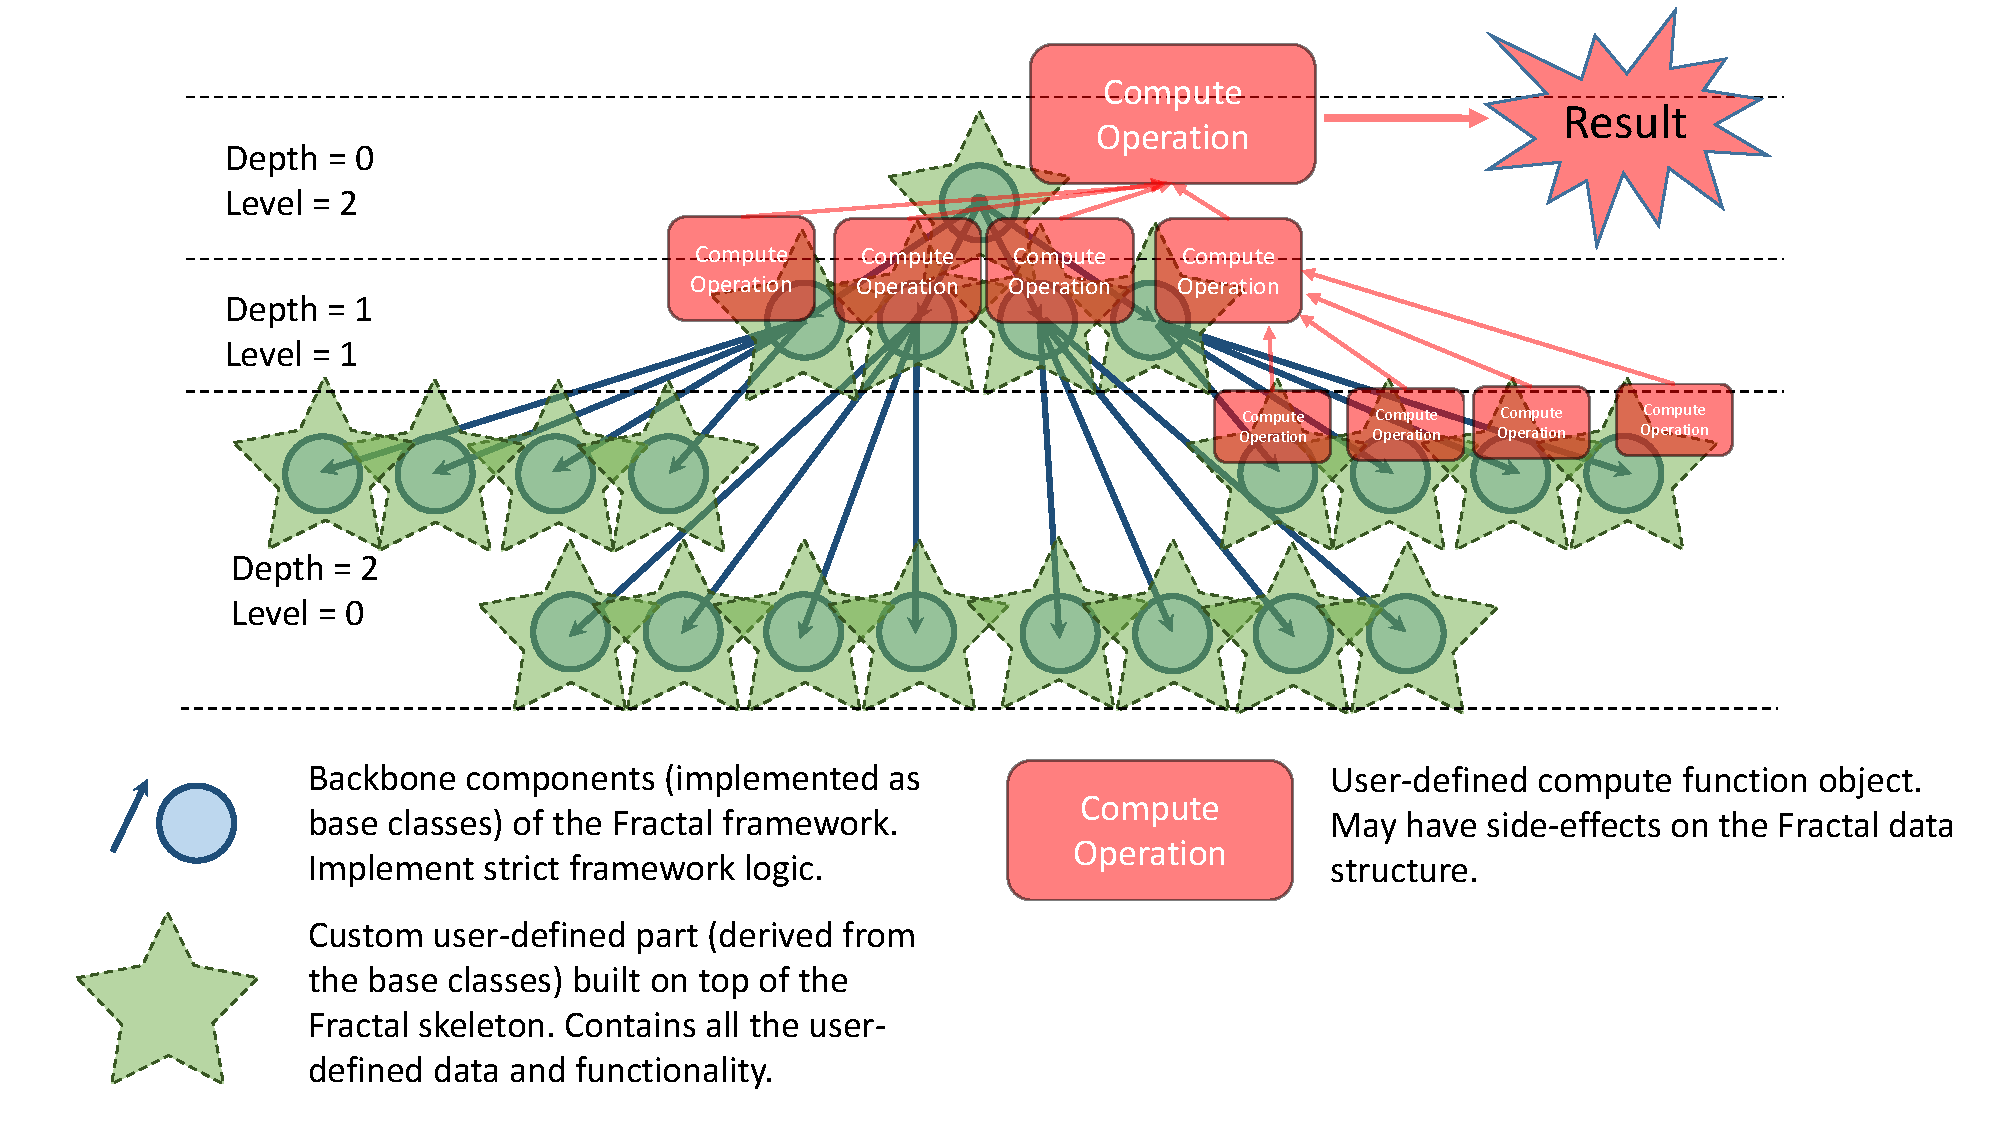
\includegraphics[width=1.0\textwidth]{images/Fractal.pdf}
\caption{The Fractal computational framework.}
\label{fig:fractal}
\end{figure}
\quad A more complicated and interesting fractal example would be a square being continuously and recursively divided into 4 equal sub-squares (southwest, northwest, southeast and northeast). The deep-growing structure is actually a 4-ary tree as well. Imagine one wants to compute the perimeter of some figure. One way to do it would be to map the figure on the square plane and then turn the plane into a grid by continuously splitting the square into 4 equal sub-parts (southwest, northwest, southeast, northeast) till we reach the granularity size of the grid. Then we paint all the grid elements located inside the figure shape as black and those outside of it as white. We iterate over the grid and detect all points of color flips and add the size of the grid elements to the final sum, which at the end is going to approximate the perimeter of the figure. That is roughly what the perimeter benchmark does.\newline\null
\quad In all its generality the fractal is a pattern, which can be characterized with self-similarity, repeatedness, structuredness, inherent parallelizability and the exact numeric values such as its depth and arity. All that naturally maps onto the C++ implementation as a class template we describe below.
\subsection{Fold}
\quad The Fold computational framework has been inspired by the computation done in the power benchmark. The fold is not a new concept and has found a wide application in many functional languages. The C++ language provides std::accumulate() function template as a component of its Standard Template Library, which performs a functional fold over a given data structure, but contrary to our computational framework does not allow any side-effects and modifications to the elements of the data structure. Moreover, our C++ class template library provides an alternative interface to a user with an extensible customization space.\newline\null
\begin{figure}[ht]
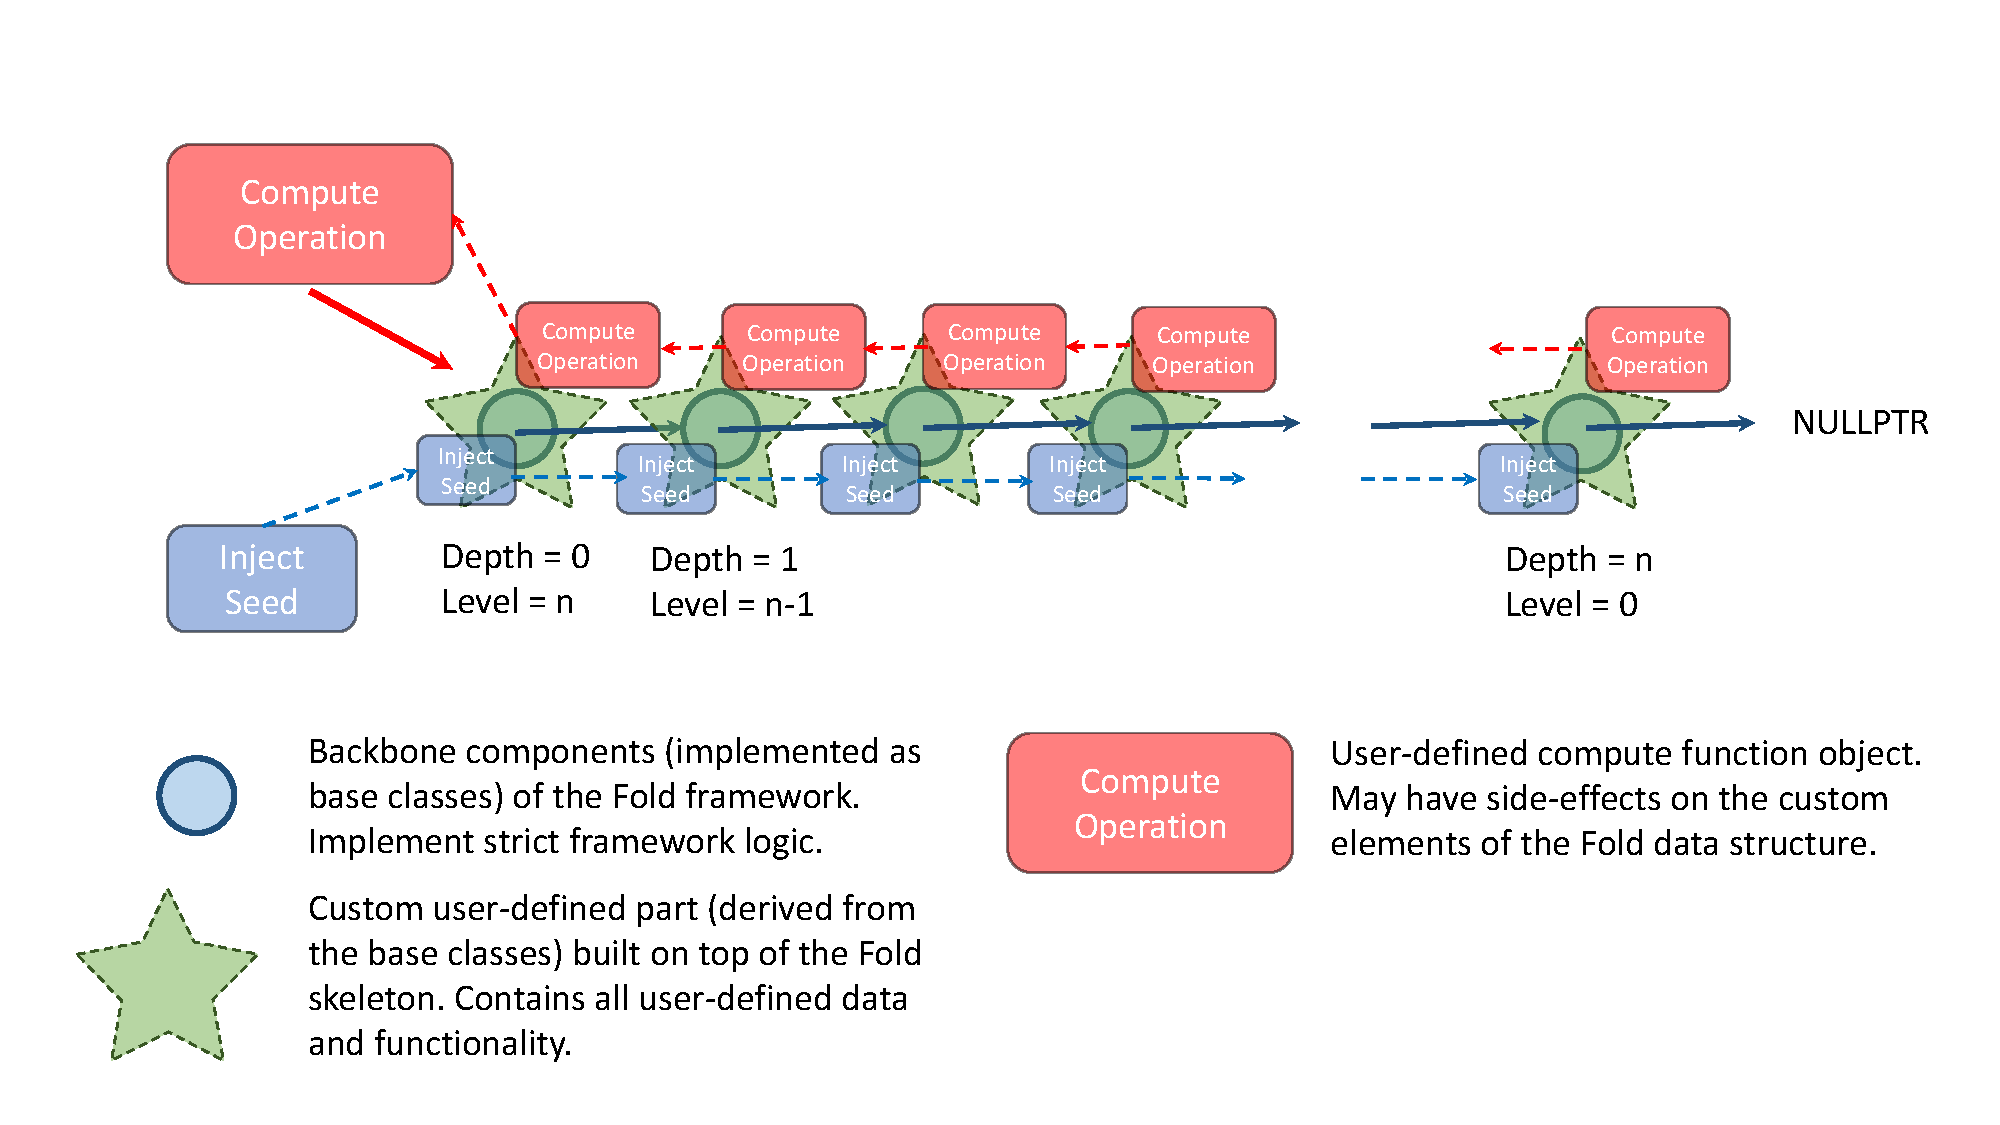
\includegraphics[width=1.0\textwidth]{images/Fold.pdf}
\caption{The Fold computational framework.}
\label{fig:fractal}
\end{figure}
\quad One can think of a Fold as a set of elements arranged into a linked-list. We grow the list to the specified depth given a seed value. Then we may inject some data into the head of the list and propagate it to its tail element. All propagation modifications are user-defined. Once every element of the list is ready with its data, the computation starts at the tail element and passes computed values back to previous elements of the chain.         


\subsection{Reduce}
\quad The Reduce computational framework is a well-known one. The difference between our computational framework and std::reduce() from C++ Standard Template Library (STL) is the possibility of having side effects and an alternative user customization interface. Our computational framework takes a function object with two overloaded and overridden virtual operator() methods. One specifies how to reduce the value from a single element (possibly changing the element in the process) and the other one defines the way of combining all the reduced values into the final return value. Our framework implements sequential as well as parallel Reduce versions.  


\subsection{Frameworks Library Design and Implementation}
\quad The design and implementation of computational frameworks library have been done iteratively using 4 Olden benchmarks as inspiration and  
The design of the C++ computational frameworks library aims at several goals.  
\begin{description}
\item[Modern C++] The implementation of the library is based on the Standard Template Library (STL) data structures, uses move semantics and unique pointers to achieve efficiency and smart memory management. For parallelization library uses OpenMP standard. All that provides for a wide source-code portability. The library is composed of a set of header files with class templates, which are supposed to be included into the user application.  
\item[Convenience] 
\item[Coherence] All computational frameworks in the library share the same user interface as well as internal design. Frameworks are inter-operable and flexible: one can create say, a fold of fractals of reductions. Different components can compute different return types.

\item[Sound design] CRTP, Algorithm Template pattern
\end{description}
\quad The computational frameworks are designed as a set of C++ class templates. The user interface these templates provide has been designed and refined iteratively using the set of Olden benchmarks [].     

\begin{minipage}[t]{\linewidth}
\begin{lstlisting}[caption={Computational framework class template skeleton},label={lst:framework_template_skeleton},language=C++]

template <typename ElemType, typename SeedType>
class Framework {
    public:
        class Element {
            // user-exposed customization iface
            virtual void grow(SeedType) = 0;
            virtual bool growth_stop_condition() { return false; }
        };
        template <typename ComputeType>
        class ComputeFunction {
            // framework specific application function API
            virtual operator()(ElemType& elem, ... ) = 0;
            virtual operator(const std::vector<ComputeType>&) = 0;
*       };
   /     
        void grow(size_t size, SeedType seed) {
            // organise framework elements 
            // into a data structure
            ... = new ElemType(); 
        }
        template<typename ComputeType>
        ComputeType compute(ComputeFunction<ComputeType>& apply_func);
    
    private:
        // framework data structure organisation
        // (list, tree, array, etc.)
};

\end{lstlisting}
\end{minipage}

\quad The design and the implementation of our template library reflect the target goals of the concept of computational frameworks.    

\quad There were several questions raised in the design process of a template library. 

\section{Performance of the library}
\quad We have rewritten old legacy C implementations of 4 Olden benchmarks: health, perimeter, treeadd and power. The table below shows the performance gains our versions have over old sequential implementations.

\section{SPEC CPU2006 Feasibility Study}


\section{DCP plan}
\quad I am planning to work solely on the DCP project throughout the second year of my PhD. This section very roughly approximates the plan I am going to follow.

\begin{description}[style=nextline]
\item [Detailed Literature Review] Get into the details of currently available dynamic data structure recognition tools (like MemPick, DDT, ARISTE, DSI, DSIbin, HeapDbg, DsOli, etc.). The detailed study will help me see the current deficiencies of these tools, competing techniques they use, the results they manage to achieve. 

\item [Technical Implementation Planning] In this stage I would need to choose the exact libraries and frameworks I will use as the base for the implementation of my data structure recognition tool. Currently I am looking at Pin and LLVM. Pin is a dynamic binary instrumentation framework for the IA-32, x86-64 and MIC instruction-set architectures that enables the creation of dynamic program analysis tools. Alternatively, instrumentation can be done at LLVM IR level.

\item [The Search of Suitable Benchmarks] SPEC CPU2006 benchmarks proved to be difficult for automatic (and even manual) data structure recognition. Maybe MCF benchmark could be used for an attempt to dynamically recognize a tree like data structure, but for a more feasible result we would need to find simpler benchmarks. SNU NPB benchmarks do not contain any data structures but linear arrays. A study of Olden benchmarks could be conducted. There has been proposed an idea of searching GitHub through its API for a simpler examples being from a real world at the same time. Alternatively Rodinia and Parboil benchmark suites might be used for a study.

\item [Memory Graph Construction] In this task we need to determine the exact way we are going to build a graph. The types of nodes and the way we connect them. Majority of tools like DDT \cite{1669122} use heap allocated nodes as memory graph composing elements. On the contrary Data Structure Investigator (DSI) tool \cite{Rupprecht:2017:DID:3155562.3155607} uses strands (abstractions over a linked list data structure) as primitives chasing recognition of Linux kernel CDLL list of different element types. The task is similar to the task of compiler's Intermediate Representation (IR) design and is going to affect all other stages.

\item [Memory Graph Analysis] Once the memory graph corresponding to some particular instance of dynamic program execution is built, the task is to recognize a data structure the graph might correspond to. The current techniques examine the properties of memory graphs (the number of edges per node, cycles, connectivity, etc.), try to apply machine learning and clustering techniques in order to learn to recognize  
\item [Data Structure Replacement] This is the most ambitious goal one might dream to achieve. Neither of all available tools has managed to do that. The task is to detect and replace unsuccessfully chosen data structure variants with a better suited one (like AVL tree instead of a binary search tree).   

\end{description}

\printbibliography

\end{document}